\documentclass{article}
\usepackage[utf8]{inputenc}
\usepackage{graphicx}
\usepackage[left=3cm, right=4cm, top=2cm]{geometry}


\title{\textbf{Trabajo tutelado BD \\ ------ \\ Logística de un campeonato de boxeo}}

\author{David Rodríguez Bacelar}
\date{\today}

\begin{document}

\maketitle

\section{Memoria y especificación del dominio}
Se realizaron las siguientes suposiciones con respecto al dominio inicial:
\begin{enumerate}
	\item Es necesario guardar un \textbf{historial de clubes} por los que pasó un boxeador para
		conocer en cual de ellos estaba afiliado en un determinado campeonato.
	\item Un campeonato puede no tener ningún club inscrito y, en consecuencia, ningún combate celebrado.
	\item Cada \textbf{club}, \textbf{campeonato} y \textbf{combate} tendrá un identificador único; los \textbf{jueces} y 
		los \textbf{boxeadores} se identificarán por su DNI; y el \textbf{recinto} por su nombre.
	\item Es necesario registrar los combates en la base de datos antes de que se celebren, por lo que el atributo \textit{ganador}
		tiene que poder ser nulo.
	\item Todo combate se celebra en una competición.
	\item Cada combate tiene que tener un recinto asociado donde se celebra, pero no tiene por qué tener ninguna zona asociada.
	\item Los jueces \textbf{no} son los encargados de poner las faltas en los combates.
	\item Aunque el atributo categoría podría ser derivado (obteniéndose a través del peso del boxeador), por la importancia que este tiene
		y para no complicar aún más la base de datos, no lo será.
\end{enumerate}

\smallskip
Con respecto a la modelización, se descartó la opción de establecer un orden en las tablas, esto es, que el \textit{Boxeador 1} tuviera las faltas
que cometió en la columna \textit{Faltas 1} y sus puntuaciones en la columna \textit{Puntuación 1}. Esto provoca que, al no saber a 
priori si un boxeador determinado es el 1 o el 2, se tengan que hacer dos consultas sql para encontrar los datos que buscamos.
Aunque esto último se podría solucionar con un UNION, en mi opinión se complicaría en exceso una consulta que debería ser mucho más sencilla.

\smallskip
Por ello, se eligió complicar quizá un poco más el diseño de la base de datos a costa de facilitar las consultas construyendo dos
nuevas relaciones:
\begin{itemize}
	\item \textbf{Comete faltas}: Donde para cada boxeador y asalto determinado se almacene el número de faltas cometidas.
	\item \textbf{Puntúa}: Donde para cada boxeador, asalto y juez determinado se almacenen los puntos obtenidos por dicho boxeador.
\end{itemize}

\smallskip
Por otra parte, también se buscó restringir que un boxeador sin equipo o que no perteneciera a ningún club inscrito a un campeonato
determinado puediera combatir, pero complicaba demasiado el diseño.

\bigskip\bigskip\bigskip\bigskip\bigskip
\section{Diagrama Entidad-Relación}
\bigskip\bigskip\bigskip
\begin{figure}[h!]
	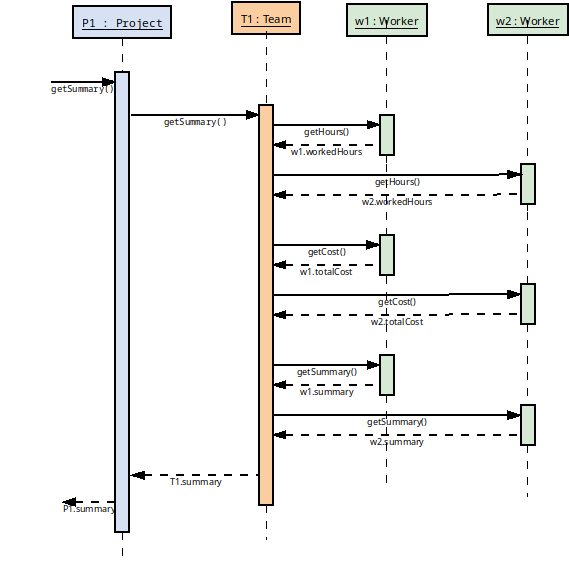
\includegraphics[height=250px]{Diagram1.pdf}
\end{figure}

\newpage
\section{Esquema Relacional}
\begin{figure}[h!]
	\includegraphics[height=600px]{Entidad_Relación.pdf}
\end{figure}

\end{document}
